\documentclass[11pt]{article}
\usepackage{latexsym}
\usepackage{amsmath}
\usepackage{amssymb}
\usepackage{amsthm}
\usepackage{epsfig}
\usepackage[tight]{subfigure}
\usepackage{graphicx}
\graphicspath{ {./imgs/} }
\usepackage{amsmath}

\DeclareMathOperator*{\minimize}{min}
\DeclareMathOperator*{\maximize}{max}

\usepackage{algorithm}
 %on linux you may need to run sudo apt-get install texlive-full to install algorithm.sys
\usepackage{algorithmic}

\usepackage{verbatim}

\newcommand{\handout}[5]{
  \noindent
  \begin{center}
  \framebox{
    \vbox{
      \hbox to 5.78in { {#1} \hfill #2 }
      \vspace{4mm}
      \hbox to 5.78in { {\Large \hfill #5  \hfill} }
      \vspace{2mm}
      \hbox to 5.78in { {\em #3 \hfill #4} }
    }
  }
  \end{center}
  \vspace*{4mm}
}
\newcommand{\specialcell}[2][c]{%
  \begin{tabular}[#1]{@{}c@{}}#2\end{tabular}}
  
\newcommand{\lecture}[5]{\handout{#1}{#2}{#3}{#4}{#5}}
\newcommand{\collision}[0]{\mathrm{collision}}
\newcommand{\nocollision}[0]{\overline{\collision}}

\newcommand*{\QED}{\hfill\ensuremath{\square}}

\newtheorem{theorem}{Theorem}
\newtheorem{corollary}[theorem]{Corollary}
\newtheorem{lemma}[theorem]{Lemma}
\newtheorem{observation}[theorem]{Observation}
\newtheorem{proposition}[theorem]{Proposition}
\newtheorem{definition}[theorem]{Definition}
\newtheorem{claim}[theorem]{Claim}
\newtheorem{fact}[theorem]{Fact}
\newtheorem{assumption}[theorem]{Assumption}
\newtheorem{note}[theorem]{Note}

% 1-inch margins, from fullpage.sty by H.Partl, Version 2, Dec. 15, 1988.
\topmargin 0pt
\advance \topmargin by -\headheight
\advance \topmargin by -\headsep
\textheight 8.9in
\oddsidemargin 0pt
\evensidemargin \oddsidemargin
\marginparwidth 0.5in
\textwidth 6.5in

\parindent 0in
\parskip 1.5ex
%\renewcommand{\baselinestretch}{1.25}

\begin{document}

\lecture{Statistical Techniques in Robotics (16-831, S22)}{Lecture \#06
  (Monday, February 7)}{Lecturer: Kris Kitani}{Scribes: Jinkun Liu, Thomas Xu}{Online Convex Optimization (Convexity, FTL)}

\section{Review}
In the last lecture, on the topic of Online Linear Classification, we formalized the linear classification problem and analyzed two approaches to learning an online linear classifier: the Perceptron algorithm and the Winnow algorithm. As a quick recap, the Perceptron algorithm uses additive updates whereas the Winnow algorithm uses multiplicative updates to the model weights each timestep. After the review section, we cover online convex optimization, which is a generalization of online learning problems like online classification and online experts, and introduce the Follow the Leader algorithm which is a general method for online optimization problems.

%This section serves as a review of the previous lecture and any other context required to frame the content of the current lecture. 

%You may format the scribes in any way you like, aside from changing font style, size and page format. Please use subsections and paragraphs to increase the readability of your notes.

%Length requirement 1-2 pages.

%%%%%%%%%%%%%%%%%%%%%%%%%%%%%%%%
%%%%% Online Linear Classification
%%%%%%%%%%%%%%%%%%%%%%%%%%%%%%%

\subsection{Online Linear Classification}
Online linear classification is a form of supervised learning; the learner trains on samples that are received online and iteratively learns to classify them correctly. There are many real-world applications of these types of problems, such as a quality assurance system to identify faulty products in an assembly line, or an agricultural robot learning to differentiate different kinds of fruit.
% could add some links/refs here if needed

The inputs to online linear classification problems are typically denoted by $\boldsymbol{x}^{(t)}$, where the superscript indicates the timestep. These inputs are vectors, whose elements or "features" may be either continuous (e.g. weight, size) or binary (e.g. stamped, purple). The outputs of the learner at each timestep are its classification predictions, which are typically denoted by $\hat{y}^{(t)}$. Similarly, the true label or correct classification is denoted by $y^{(t)}$ or $y^t$.

Linear classification of the samples is achieved using hyperplanes, which are defined such that "positive" samples satisfy the following inequality:
\begin{align}
    \boldsymbol{w}^{(t)} \cdot \boldsymbol{x}^{(t)} \geq N \quad\quad \boldsymbol{w}^{(t)} \in \mathbb{R}^N, \boldsymbol{x}^{(t)} \in \mathbb{R}_+^N
\end{align}
Here, $w^{(t)}$ indicates the parameters of the hyperplane. $N$ is a threshold value that can be set arbitrarily. If a sample does not satisfy the above inequality, then it will be classified as "negative." In other words, the prediction rule of the hyperplane is given by:
\begin{align}
    \hat{y}^{(t)} = \text{sign}(\boldsymbol{w}^{(t)} \cdot \boldsymbol{x}^{(t)} - N)    
\end{align}


%%%%%%%%%%%%%%%%%%%%%%%%%%%%%%%%
%%%%% perceptron
%%%%%%%%%%%%%%%%%%%%%%%%%%%%%%%
        
\subsection{Perceptron Algorithm}
The Perceptron algorithm is an online linear classification learning algorithm that makes predictions using the sign of a dot product between its learned weights and the received feature vector. It learns the weights after making mistakes using additive updates based on the true labels received.  

\begin{algorithm}[H]
\caption{Perceptron algorithm}
\label{algo:perceptron}
\begin{algorithmic}[1]
\STATE $\textbf{w}^{(1)} \leftarrow 0$ \hfill $\triangleright$ Initialize weights
\FOR{$t=1,\;\cdots,\;T$}
\STATE \textsc{Receive} ($\textbf{x}^{(t)}\in \mathbb{R}^N$) \hfill $\triangleright$ Receive feature vector
\STATE $\hat{y}^{(t)} = \text{sign}\Big(\langle \textbf{w}^{(t)}, \textbf{x}^{(t)}\rangle \Big)$ \hfill $\triangleright$ Predict label
\STATE \textsc{Receive} ($y^{(t)}\in\{-1, 1\}$) \hfill $\triangleright$ Receive true label
\STATE $\textbf{w}^{(t+1)}\leftarrow \textbf{w}^{(t)} + y^{(t)} \cdot \textbf{x}^{(t)} \cdot\textbf{1}[y^{(t)}\neq \hat{y}^{(t)}] $ \hfill $\triangleright$ Update weights
\ENDFOR
\end{algorithmic}
\end{algorithm}

One benefit of the Perceptron algorithm is speed, as its prediction and weight update entails only a dot product and an addition respectively. However, it is not a large margin classifier as it only uses sign to make decisions, and does not use any notion of associated distance or margin. Furthermore, the Perceptron algorithm will not converge and stop making mistakes if the data isn't linearly separable, since its decision boundary is a hyperplane.
For linearly separable data, the Perceptron algorithm's mistake bound \cite{novikoff1963convergence} is 
\begin{align}
    M \leq \frac{R^2}{\gamma^2}   
\end{align}
Here, $R=\max\limits_t \|x^{(t)}\|$ is the infinity norm of data examples and $\gamma=\min\limits_t y_t \langle \textbf{w}^\star, \textbf{x}^{(t)} \rangle$ is the data's margin of separability.

%%%%%%%%%%%%%%%%%%%%%%%%%%%%%%%%
%%%%% winnow (review)
%%%%%%%%%%%%%%%%%%%%%%%%%%%%%%%

\subsection{Winnow Algorithm (Introduction)}
The Winnow algorithm is an online linear classification algorithm that operates on binary features as inputs. The name ``winnow" originally came from the term ``winnowing," which is the act of shaking or blowing air through a bundle of grain to remove unnecessary parts (``chaff" or ``husks").
The key assumption of the Winnow algorithm is that only a certain subset of the features are relevant for classification. Specifically, the algorithm assumes that a perfect hypothesis $h^\star$ is a disjunctive Boolean function \cite{littlestone1988winnow} of the form
\begin{align}
    h^\star(\boldsymbol{x})=x_{n,1}\;\vee\cdots\vee x_{n,K}
\end{align}

where $\boldsymbol{x}$ is a vector of binary features and $K$ is the number of relevant features. The Winnow algorithm uses the following equation to predict labels:
\begin{align}
    \hat{y}^{(t)} = \boldsymbol{1}\left[\langle\boldsymbol{w}^{(t)},\boldsymbol{x}^{(t)}\rangle > \Theta\right]
\end{align}

Here, $\Theta$ is the threshold that is used to define the decision boundary (hyperplane). The details of Winnow algorithm will be discussed in Section \ref{sec:winnow_algo}.


\section{Summary}
\subsection{Winnow Algorithm (Weight Update and Mistake Bound)}
\label{sec:winnow_algo}
As mentioned in the review section, the Winnow algorithm is an approach that can be used for online linear classification problems. It is similar to the Perceptron algorithm, and also classifies examples using a hyperplane, but has some notable differences. For instance, the Winnow algorithm uses multiplicative instead additive weight updates, and does not always use a threshold of zero.

The input to the Winnow algorithm is denoted by $\boldsymbol{x}$, which is a vector of binary features:
\begin{align}
    \boldsymbol{x} = \{x_1, \dots, x_N\}, \quad x_n \in \{0,1\}
\end{align}

As discussed in the review section, the Winnow algorithm assumes that the perfect hypothesis ($h^*$) is a disjunctive Boolean function. Note that the weights ($w_n$) in the Winnow algorithm are always non-negative, and that the weights are initialized to 1 (instead of 0, as in the Perceptron algorithm).


\begin{algorithm}[H]
\caption{Winnow algorithm}
\label{algo:winnow}
\begin{algorithmic}[1]
\STATE $\textbf{w}^{(1)} \leftarrow \{1,...,1\}$ \hfill $\triangleright$ Initialize weights
\FOR{$t=1,\;\cdots,\;T$}
\STATE \textsc{Receive} ($\textbf{x}^{(t)} \in\{0, 1\}^N$) \hfill $\triangleright$ Receive feature vector
\STATE $\hat{y}^{(t)} = \textbf{1}[\langle \textbf w^{(t)}, \textbf x^{(t)}\rangle>\Theta]$ \hfill $\triangleright$ Predict label
\STATE \textsc{Receive} ($y^{(t)}\in\{0, 1\}$) \hfill $\triangleright$ Receive true label
\STATE $w_n^{(t+1)}\leftarrow w_n^{(t)} (1+\beta)^{ (y^{(t)}-\hat{y}^{(t)})\cdot x_n^{(t)}} $ \hfill $\triangleright$ Update weights
\ENDFOR
\end{algorithmic}\label{algo:winnow}
\end{algorithm}


As seen in the above algorithm (line 6), the Winnow weight update rule is given by:
\begin{align}
    w_n^{(t+1)}\leftarrow w_n^{(t)} (1+\beta)^{ (y^{(t)}-\hat{y}^{(t)})\cdot x_n^{(t)}}
\end{align}
Here, $\beta$ is a constant parameter that affects the magnitude of weight updates. A typical value \cite{littlestone1988winnow} is $\beta=1$. Note that the $(1+\beta)$ term may be given in different forms. For example, other papers may replace that term with $e^\eta$ or $\alpha$ \cite{littlestone1988winnow}.

From the expression in the exponential in the update rule, we can observe that weight updates are only performed when mistakes are made ($y^{(t)} \neq \hat{y}^{(t)}$), and only for weights corresponding to the positive input features ($x_n=1$). Additionally, the direction of weight updates depend on the type of mistakes made. This is summarized in Table \ref{tab:Weight Update} below.

\begin{table}[!htbp]
\caption{\label{tab:Weight Update}Winnow updates weights depending on the type of mistake.}
\centering
\begin{tabular}{|c|c|c|c|c|c|}
\hline
\specialcell{Label\\($y^{(t)}$)} & \specialcell{Prediction\\($\hat{y}^{(t)}$)} & \specialcell{Gain\\(${y}^{(t)}-\hat{y}^{(t)}$)}& \specialcell{Type of Mistake}       & \specialcell{Weight Update} & \specialcell{Update Name \cite{littlestone1988winnow}} \\ \hline
0    & 1       & -1   & Mistake on Negative    & Decrease by $\frac{1}{(1+\beta)}$ & Demotion Step   \\ \hline
1    & 0      & 1     & Mistake on Positive    & Increase by  $(1+\beta)$ & Promotion Step \\ \hline
\end{tabular}
\end{table}

% \subsubsection{Mistake Bound}
\paragraph{Mistake Bound}Let $M$ be the total number of mistakes made by the learner using the Winnow algorithm. Assuming $\beta=1$, then $M$ is upper-bounded as:
\begin{align}
    M<2+3k({\log_2 N+1})
\end{align}

where $N$ is the total number of input features and $k$ is the number of relevant features. The derivation of this mistake bound can be found in the Appendix.

% % To derive the mistake bound of the Winnow algorithm, we must handle the two types of mistakes (positive and negative) separately.

\normalfont


\subsection{Online Convex Optimization}

Online convex optimization serves as a generalized framework of many online tasks, including the online learning problem covered in previous lectures. It was first formalized in 2003 by Zinkevich \cite{zinkevich2003OnlineCP}. In summary, an online convex optimizer interacts with nature by producing predictions using its parameters $\boldsymbol{w}^{(t)}\in \mathcal{S}$, and receiving loss function ${l}^{(t)}$ from nature that it will use to update its parameters. Here, $\mathcal{S}$ must be a convex set and ${l}^{(t)}$ must be a convex function; we will cover these concepts later in this section. The diagram in Figure \ref{fig:convex_optim} demonstrates this framework:

\begin{figure}[h]
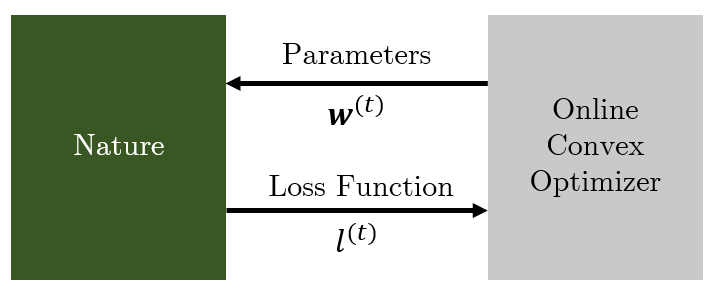
\includegraphics[scale=0.5]{imgs/convex_optim.png}
\centering
\caption{Online convex optimizer's interaction with nature.}
\label{fig:convex_optim}
\end{figure}
% \begin{enumerate}
%     \item A data sample is received from nature
%     \item A prediction is made based on the data sample
%     \item The loss function is received from nature
%     \item The optimizer's parameters/weights are updated based on the loss
%     \item (Repeat)
% \end{enumerate}
There are two ways to interpret how online convex optimization is a 
generalization of online learning:
\begin{enumerate}
    \item An online learner with convex loss can be viewed as part of the nature that the online convex optimizer interacts with.
    \item The online convex optimizer can be viewed as the update method for an online learner with convex loss.
\end{enumerate}
Figure \ref{fig:oco} below illustrates both interpretations.
\begin{figure}[h]
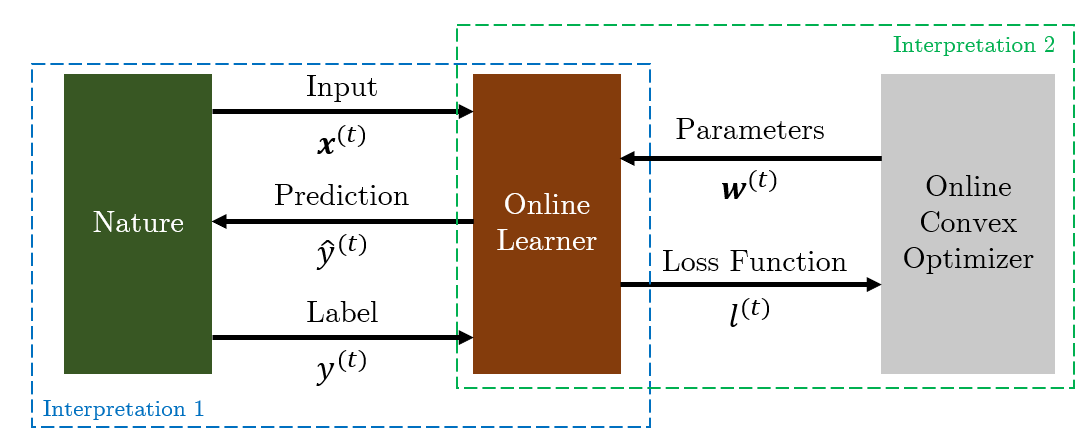
\includegraphics[scale=0.5]{imgs/oco_ol.png}
\centering
\caption{Two ways to interpret online convex optimization as a generalization of online learning.}
\label{fig:oco}
\end{figure}

\paragraph{Convex Set} A set $\mathcal{S}$ is considered a convex set if for all $\boldsymbol{w}, \boldsymbol{v} \in \mathcal{S}$:
\begin{align}
    \alpha \boldsymbol{w} + (1 - \alpha) \boldsymbol{v} \in \mathcal{S} \quad \quad \forall \alpha \in [0,1]
\end{align}
% \begin{equation*}
%     \alpha \boldsymbol{w} + (1 - \alpha) \boldsymbol{v} \in \mathcal{S} \quad \quad \forall \alpha \in [0,1]
% \end{equation*}
In other words, the points that lie linearly between $\boldsymbol{w}$ and $\boldsymbol{v}$ must all also be inside $\mathcal{S}$. The $\alpha$ term indicates how far along a given point is between $\boldsymbol{w}$ and $\boldsymbol{v}$ (e.g. $\alpha=1$ means the point is at $\boldsymbol{w}$, and $\alpha=0.5$ means the point is halfway between $\boldsymbol{w}$ and $\boldsymbol{v}$). Figure \ref{fig:convex_sets} provides numerical and geometrical examples of convex and non-convex sets.

\begin{figure}[h]
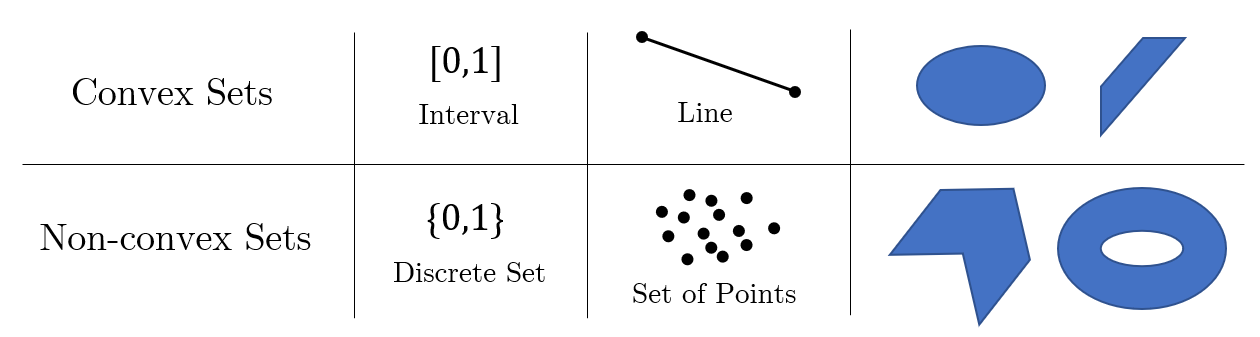
\includegraphics[scale=0.5]{imgs/convex_sets.png}
\centering
\caption{Examples of convex and non-convex sets.}
\label{fig:convex_sets}
\end{figure}

\paragraph{Convex Function}
A function $f : \mathcal{S} \rightarrow \mathbb{R}$ is considered a convex function if for all $\boldsymbol{w}, \boldsymbol{v} \in \mathcal{S}$:
\begin{align}
    f(\alpha \boldsymbol{w} + (1 - \alpha) \boldsymbol{v}) \leq \alpha f(\boldsymbol{w}) + (1 - \alpha) f(\boldsymbol{v}) \quad \quad \forall \alpha \in [0,1]
    \label{eqn:convex_func}
\end{align}
The interpretation of this definition is as follows: the right-hand side of the inequality forms a straight line between two points $f(\boldsymbol{w})$ and $f(\boldsymbol{v})$. All points on this line must be above or equal to the function itself across the same interval, for the function to be convex. Figure \ref{fig:convex_func} illustrates this interpretation.
Additionally, a function is \textbf{strictly convex} if the inequality in Equation \ref{eqn:convex_func} holds strictly (i.e., $<$ rather than $\leq$) for all $\alpha \in (0,1)$ and $\boldsymbol{w}\neq\boldsymbol{v}$.
\begin{figure}[h]
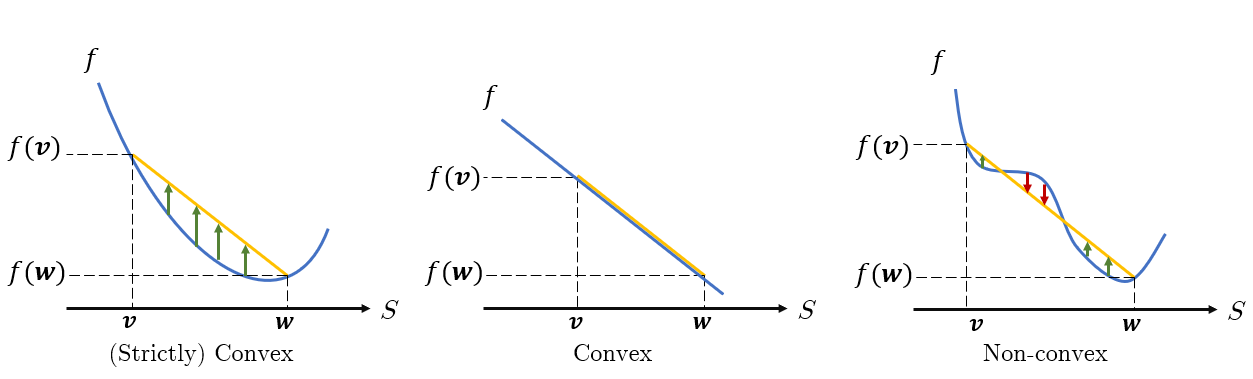
\includegraphics[width=\textwidth]{imgs/convec_func.png}
\centering
\caption{Examples of convex and non-convex functions. The function is convex if the yellow line connecting $f(\boldsymbol{w})$ and $f(\boldsymbol{v})$ is entirely above or on the function itself, for all $\boldsymbol{w}, \boldsymbol{v} \in \mathcal{S}$.}
\label{fig:convex_func}
\end{figure}


\paragraph{Lipschitz Continuity}
A function $f(\cdot)$ is called ``L-Lipschitz" over a set $\mathcal{S}$ with respect to a norm $|| \cdot ||$ if:
\begin{equation}
    \label{eq:lipschitz}
    |f(\boldsymbol{u}) - f(\boldsymbol{w})| \leq L || \boldsymbol{u} - \boldsymbol{w} || \quad \quad \forall \boldsymbol{u}, \boldsymbol{w} \in \mathcal{S}
\end{equation}
Here, $L$ is the ``Lipschitz constant." Any standard norm or distance function can be used here, such as the L-2 norm. This expression essentially sets a bound on the function's rate of change: the left side is the function value difference or ``rise" between two points ($\boldsymbol{u}$ and $\boldsymbol{v}$), and the right side (without the Lipschitz constant) is the input value difference or ``run." Also, note that this expression can also be used to show that compositions of Lipschitz functions are also Lipschitz functions \cite{wu2019convex}: if $f(x) = g(h(x))$, where $g(x)$ is $L_1$-Lipschitz and $h(x)$ is $L_2$-Lipschitz, then $f(x)$ is $L_1L_2$-Lipschitz.

As discussed earlier, performing convex optimization requires both a convex function and a convex solution space. For learning problems, this typically means that the hypothesis class must be a convex set with elements with bounded magnitudes and the loss function must be a convex function. Note that in order for the optimization to actually be solved, the function must also be L-Lipschitz. Together, these conditions are sufficient to form a ``Convex-Lipschitz-Bounded" learning problem. 

Another similar class of learning problems that can be solved with convex optimization is ``Convex-Smooth-Bounded" learning problems, where the function is ``convex-smooth" instead (see Appendix).

\paragraph{Convexification}
Certain methods can be employed to convert non-convex problems into convex ones, typically by converting a non-convex loss function into a convex one.

One method is convexification by \textbf{randomization}. By adding randomness to an algorithm, its loss function may be changed from a non-convex one to a convex one. For example, the Weighted Majority Algorithm (WMA) has a loss function given by:
\begin{align}
    l^{(t)} = \mathbf{1}[y^{(t)} \neq \hat{y}^{(t)}]
\end{align}
This loss function forms the shape of a step function when graphed, and is not convex. However, if we add randomization to WMA and make it the Randomized Weighted Majority Algorithm (RWMA), the random sampling changes the zero-one loss function into an expectation:
\begin{align}
    l^{(t)} = E_{\boldsymbol{p}}[\mathbf{1}[y^{(t)} \neq \hat{y}^{(t)}]]=\sum_{p_n} p_n \cdot \mathbf{1}[y^{(t)} \neq \hat{y}_n^{(t)}]
\end{align}
The probability term allows this new loss function to take on any values between 0 and 1, making it a linear and convex function.

Another method is convexification by \textbf{surrogate loss}. This method replaces the original non-convex loss function with a surrogate loss function that:
\begin{itemize}
    \item Upper-bounds the original loss function
    \item Is a convex function
\end{itemize}
This method is viable because minimizing the surrogate loss is equivalent to minimizing an upper bound on the original loss function. An example surrogate loss for WMA can be derived as below:
\begin{align}
    l^{(t)} &= \mathbf{1}[y^{(t)} \neq \hat{y}^{(t)}]\\
     &= \mathbf{1}[-y^{(t)}\hat{y}^{(t)}>0]\\
     &= \mathbf{1}[1-y^{(t)}\langle \boldsymbol{w}^{(t-1)},\boldsymbol{x}^{(t)}\rangle >1]\\
     &\leq     \text{max}\big[0,1-y^{(t)}\langle \boldsymbol{w}^{(t-1)},\boldsymbol{x}^{(t)}\rangle>1\big]\\
     \Tilde{l}^{(t)}&=\text{max}\big[0,1-y^{(t)}\langle \boldsymbol{w}^{(t-1)},\boldsymbol{x}^{(t)}\rangle>1\big]
\end{align}

The resulting surrogate loss $\Tilde{l}^{(t)}$ is known as the hinge loss, and as seen in Figure \ref{fig:hinge} below it both upper-bounds the original zero-one WMA loss and is convex. This surrogate loss function thus has transformed this problem into a convex problem.
\begin{figure}[h]
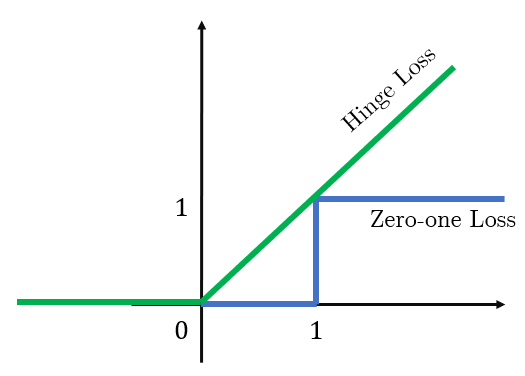
\includegraphics[scale=0.5]{imgs/hinge.png}
\centering
\caption{The non-convex zero-one loss for WMA and the convex hinge loss.}
\label{fig:hinge}
\end{figure}

\subsection{Follow the Leader}
Follow the Leader (FTL) is a generic algorithm for online (not necessarily convex) optimization problems. Its main idea is that the learner should go by the best choice in the game so far. The general pseudocode for FTL is as seen below:

\begin{algorithm}[H]
\caption{Follow the Leader}
\label{algo:FTL}
\begin{algorithmic}[1]
\FOR{$t=1,2,\;\cdots,\;T$}
\vspace{5pt}
\STATE \qquad  $\boldsymbol{w}^{(t)}=\text{arg min}_{\boldsymbol{w}\in W} \sum_{i=1}^{t-1} f^{(i)} (\boldsymbol{w})$
\vspace{5pt} \hfill $\triangleright$ Update parameter
\STATE \qquad  $\textsc{Receive}(f^{(T)}:W \rightarrow \mathbb{R})$ \hfill $\triangleright$ Receive loss
\ENDFOR

\end{algorithmic}
\end{algorithm}

Assuming a \textbf{linear} loss of the form $f^{(t)}(w)=wz^{(t)}$ and solution space $w \in S = [-1,1]$, the FTL algorithm becomes:
\begin{algorithm}[H]
\caption{Follow the Leader (Linear Loss)}
\label{algo:FTL_linear}
\begin{algorithmic}[1]
\FOR{$t=1,2,\;\cdots,\;T$}
\STATE $w^{(t)} = \text{argmin}_{w \in S} \Big(\Sigma_{i=1}^{t-1} {z}^{(i)} \Big) \cdot w$ \hfill $\triangleright$ Update parameter
\STATE \textsc{Receive} ($f^{(t)}(w)=wz^{(t)}$) \hfill $\triangleright$ Receive loss
\ENDFOR
\end{algorithmic}
\end{algorithm}

Note that in some scenarios, FTL with linear loss can have very poor performance. For example, consider the following sequence of observations in an adversarial environment:
\begin{align}
    z^{(1)}, z^{(2)}, z^{(3)},z^{(4)},z^{(5)}, \dots = -0.5, 1.0, -1.0, 1.0, -1.0, \dots
\end{align}
Consequently, the sequence of sum of observations is:
\begin{align}
    \Sigma_{i=1}^{0} {z}^{(i)}, \Sigma_{i=1}^{1} {z}^{(i)}, \Sigma_{i=1}^{2} {z}^{(i)}, \Sigma_{i=1}^{3} {z}^{(i)},\Sigma_{i=1}^{4} {z}^{(i)},\dots = 0, -0.5, 0.5, -0.5, 0.5, \dots
\end{align}
In this case, the sequence of weights that would be chosen by the FTL algorithm in order to optimize linear loss are:
\begin{align}
    w^{(1)}, w^{(2)}, w^{(3)},  w^{(4)}, w^{(5)},\dots = 0.0, 1.0, -1.0, 1.0, -1.0, \dots
\end{align}
Then, the loss that would be incurred at each timestep would be:
\begin{align}
    f^{(1)}, f^{(2)}, f^{(3)}, f^{(4)},f^{(5)},\dots = 0.0, 1.0, 1.0, 1.0, 1.0, \dots
\end{align}
As a result, the total loss of the FTL learner is 
\begin{align}
    L = \Sigma_{t=2}^{T} 1 = T-1
\end{align}
which increases linearly with time. Additionally, the learner may be compared to an expert that simply chooses $w=0$ at each timestep; this strategy incurs zero loss over time. Therefore, the regret of the FTL learner in this case is equal to its loss and also grows linearly over time ($O(T)$), which is considered poor performance.

A more preferable loss function for FTL is \textbf{quadratic} loss of the form $f^{(t)}(w)=\frac{1}{2}\Vert w-z^{(t)}\Vert^2_2$. The parameter $w$ that minimizes this sum of squared differences is simply the average value of $z^{t}$. The corresponding algorithm is given below.
\begin{algorithm}[H]
\caption{Follow the Leader (Quadratic Loss)}
\label{algo:FTL_quadratic}
\begin{algorithmic}[1]
\STATE $f^{(0)} \leftarrow 0$ \hfill $\triangleright$ Initial loss
\FOR{$t=1,2,\;\cdots,\;T$}
\STATE $w^{(t)} = \frac{1}{t-1}\Sigma_{i=1}^{t-1} {z}^{(i)}$ \hfill $\triangleright$ Update parameter
\STATE \textsc{Receive} ($f^{(t)}(w)=\frac{1}{2}\Vert w-z^{(t)}\Vert^2_2$) \hfill $\triangleright$ Receive loss
\ENDFOR
\end{algorithmic}
\end{algorithm}

% This FTL variation with quadratic loss is typically preferable to the FTL variation with linear loss, because the FTL variation with linear loss can be shown to perform very poorly in some scenarios (see example below). Additionally, i
If it is assumed that points $z$ are bounded such that $||z||^2_2 \leq L$, then the regret bound of FTL with quadratic loss can be shown to be:
\begin{align}
    \text{Regret} \leq 4L^2 \Big( \text{log}(T) + 1 \Big)
\end{align}
Note that this grows sub-linearly in $T$, making FTL with quadratic loss a no-regret algorithm. The derivation of this regret bound will be discussed in the next lecture.



%\section*{References}
%Include your references here. Please cite any resources you found useful.	
%Populate the refs.bib file or list your references manually. Be consistent in formatting!
{
\bibliography{refs}
\bibliographystyle{abbrv}
}

\newpage
\section{Appendix}
%This section provides any relevant background material that was not covered in the lectures, but was found to be useful for understanding the material. 
%For example, derivations, theory underlying techniques employed, etc. 

%Additionally, this section can summarizes applications or extensions of these techniques found in the literature. 



\subsection{Winnow Algorithm Mistake Bound Derivation}
First, choose the potential function for the Winnow algorithm (at time $t$) as the sum of all weights:
\begin{align}
    \Phi^t = \sum_n w_n^{(t)}
\end{align}
The total mistakes made by the learner is given by:
\begin{align}
    M = m^- + m^+
\end{align}
Here, $m^+$ indicates a "mistake on positive" and $m^-$ indicates a "mistake on negative" (as defined in Summary above).
Throughout this derivation, we will also assume that $\beta=1$. 

For mistakes on positives, the weights can only increase. Thus, the following holds:
\begin{align}
    \Phi^t = \Phi^{t-1} + \boldsymbol{w}^{(t-1)} \cdot \boldsymbol{x}^{(t-1)}
\end{align}
Additionally, because $\boldsymbol{w}^{(t-1)} \cdot \boldsymbol{x}^{(t-1)} \leq \Theta$ for mistakes on positives, this simplifies to:
\begin{align}
    \Phi^t \leq \Phi^{t-1} + \Theta
\end{align}
By induction, this can be restated as:
\begin{align}
    \Phi^t \leq \Theta + m^+ \Theta
\end{align}

Next, we analyze the mistakes on negatives. For these mistakes, the weights can only decrease:
\begin{align}
    \Phi^t = \Phi^{t-1} - \sum_{n: x_n^{(t)} = 1} \frac{1}{2}w_n^{t-1} \\
    \implies \Phi^t = \Phi^{t-1} - \frac{1}{2}w^{(t-1)} \cdot x^{(t-1)}
\end{align}

For mistakes on negatives, $w^{(t-1)} \cdot x^{(t-1)} > \Theta$ holds. Thus:
\begin{align}
    \Phi^t < \Theta - m^- \frac{1}{2} \Theta
\end{align}
Combining these two bounds leads to the upper bound of the potential function:
\begin{align}
    \Phi^t \leq \Theta + m^+ \Theta - m^- \frac{1}{2} \Theta
\end{align}
The lower bound of the potential is zero, because the Winnow weights are initialized to 1 and multiplicative updates are used. Combining this with the upper bound gives:
\begin{align}
    0 \leq \Theta + m^+ \Theta - m^- \frac{1}{2} \Theta
\end{align}
Rearranging this yields:
\begin{align}
    m^- < 2 + 2m^+
\end{align}

To convert this to a bound on total mistakes, we make use of two observations. First, $w_n^{(t)}=2^{m^+}$ after $m^+$ mistakes on positives. Second, $w_n^{(t)} < \Theta$ when $x_n^{(t)}=1$, otherwise it would be impossible to make a mistake on positive. Using these observations leads to:
\begin{align}
    w_n^{(t)} = 2^{m^+-1} < \Theta \\
    \implies m^+ < \text{log}_2\Theta + 1
\end{align}


Considering $k$ relevant features, and knowing that only one weight will be updated after each mistake in the worst case, yields:
\begin{align}
    m^+ < k(\text{log}_2 \Theta + 1)
\end{align}
Substituting this into our previous inequality yields an upper bound for $m^-$:
\begin{align}
    m^- < 2 + 2k(\text{log}_2\Theta + 1)
\end{align}

Recalling that the total mistakes $M= m^+ + m^-$, we obtain the final mistake bound for the Winnow algorithm:
\begin{align}
    M < 2 + 3k(\text{log}_2\Theta + 1)
\end{align}

\subsection{Convex-Smooth-Bounded Learning Problems}
These learning problems are very similar to "Convex-Lipschitz-Bounded" learning problems, which were discussed in lecture. Both types of problems define certain properties of the solution space and corresponding function(s) such that a convex optimization problem can be solved successfully.
\paragraph{Smooth Functions} A differentiable function $f : \mathbb{R}^d \rightarrow \mathbb{R}$ is $L$-smooth if its gradient is $L$-Lipschitz \cite{wu2019convex}:
\begin{equation}
    \label{eq:smooth_func}
    || \nabla f(\boldsymbol{v}) - \nabla f(\boldsymbol{w}) || \leq L || \boldsymbol{v} - \boldsymbol{w} || \quad \quad \forall \boldsymbol{v}, \boldsymbol{w} \in \mathbb{R}^d
\end{equation}
Note that it is also common for smooth functions to be defined using $\beta$ instead of $L$.

A learning problem is called a Convex-Smooth-Bounded learning problem when the following conditions \cite{wu2019convex} are satisfied:
\begin{enumerate}
    \item The hypothesis class $H$ is a convex set.
    \item $||\boldsymbol{w}|| \leq B$ for all $\boldsymbol{w} \in H$, where $B$ is a constant parameter.
    \item The loss function $l$ is convex and non-negative.
    \item The loss function $l$ is $L$-smooth.
\end{enumerate}

\end{document} % Done!


